%%%%%%%%%%%%%%%%%%%%%%%%%%%%%%%%%%%%%%%%%%%%%%%%%%%%%%%%%%%%%%%%%%%%%%%%%%%%%%%%
\twocolumn
\section{System Engineering Approach}
\label{sec1:introduction}

%citation example: \cite{c1}
\subsection{Mission Requirement Analysis}
UBC Unmanned Aircraft Systems (UAS) went through thorough research and development, design, manufacturing and testing phases to ensure a full robust system. Using the Mission Success Analysis table below, the team determined which tasks were both reachable and yielded the greatest return with justification. All tasks listed as “High” will be attempted, while “Medium” may be attempted and “Low” will not be attempted. See table 1.


\subsection{Design Rationale}
    \subsubsection{Environmental Factors}

     This year the team approached projects with a mindset of fulfilling minimum requirements for competition before building on them to expand capabilities or reliability. Long shot ideas were minimized in favor of a faster iterative design process. This resulted in working systems much earlier in the year that allowed all system level problems to arise early enough that they could be dealt with.

    Given UBC UAS’ location in the heart on Vancouver, fixed wing flight locations are limited. Several locations within 15 minutes of the team’s design space offer space for multi-rotor testing, while fixed wing testing grounds are at least 45 minutes away and require further coordination with external groups. 
    
    \subsubsection{Aircraft Choice}
    The 2019 AUVSI SUAS competition presents a very unique engineering challenge in terms of distance, time, and accuracy requirements of the chosen aircraft design. Given the mission requirements for 6+ miles of flight and high accuracy payload drop it was determined that the most capable system for mission success would likely be some sort of VTOL. UBC UAS instead opted for a multirotor on the basis of significantly improved payload drop accuracy, easier testing, and simpler obstacle avoidance routing. Previous experience with VTOL development proved that it was not ideal to focus all efforts on such a long shot and instead to focus on reliability as stated above. This presented a number of other challenges in order to meet mission distance and time requirements. 


    \begin{figure*}\centering
    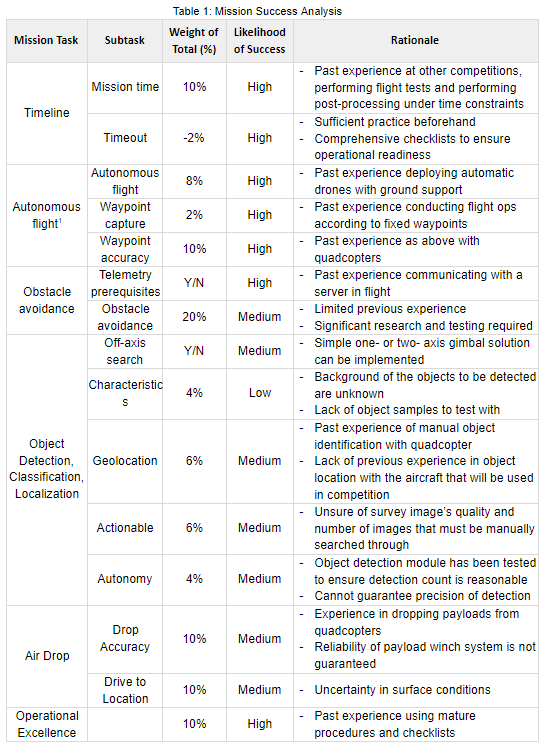
\includegraphics[width=0.9\textwidth]{table/table_1.png}
    \caption*{}
    \label{fig:msa}
    \end{figure*}



\endinput
%%%%%%%%%%%%%%%%%%%%%%%%%%%%%%%%%%%%%%%%%%%%%%%%%%%%%%%%%%%%%%%%%%%%%%%%%%%%%%%%